
\section{Programaci�n lineal}

\subsection{Programaci�n lineal}

\begin{frame} 
\frametitle{Programaci�n lineal}

Buscamos maximizar/minimizar una funci�n objetivo sujeta a un conjunto de restricciones lineales sobre las variables.

Por ejemplo, dadas $x, y \in \Re$...

\begin{align*}
\text{{maximizar}} \quad & x + y \\
\text{{sujeto a}} \quad & x + 4y \leq 16 \\
& 3x + y \leq 15 \\
& x, y \in \Re^{\geq 0}
\end{align*}

\end{frame} 

\begin{frame} 
\frametitle{Programaci�n lineal}

Las restricciones determinan una regi�n factible sobre la que se busca el �ptimo que maximiza la funci�n objetivo.

\begin{figure}[h]
	\centering
	\alt<1>{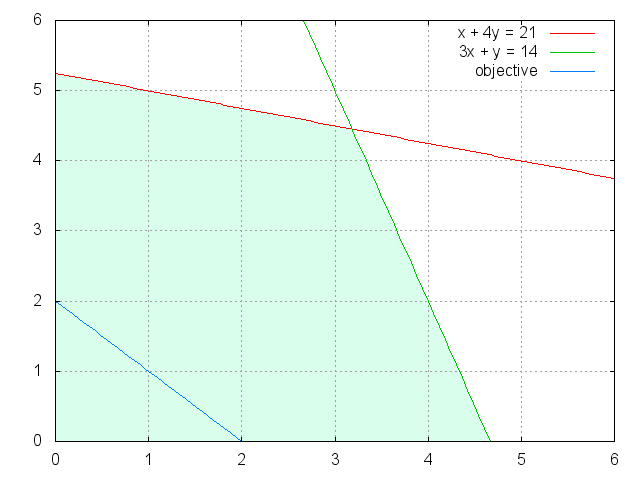
\includegraphics[scale=0.5]{lpsample1.png}}{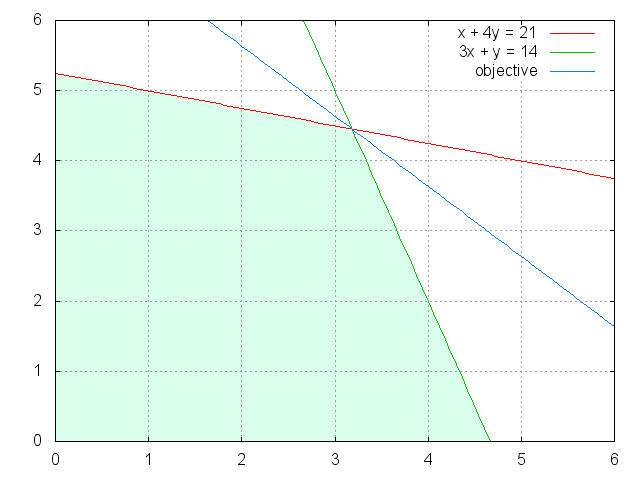
\includegraphics[scale=0.5]{lpsample2.png}}
\end{figure}

\uncover<2>{}

\end{frame}

\begin{frame} 
\frametitle{Modelado}

Podemos usar programaci�n lineal para modelar m�ltiples escenarios, sean de econom�a, planificaci�n, etc.

Intentemos usarlo para modelar implicaciones l�gicas: cada variable toma valores $0$ si es falsa o $1$ si es verdadera:

\begin{align*}
\text{maximizar} \quad & x + y + z\\
\alt<1>
{\text{sujeto a} \quad & x \xor y \\
& x \xor z \\
& y \xor z \\
& x, y, z \quad \text{bool} \\}
{\text{sujeto a} \quad & x + y \leq 1 \\
& x + z \leq 1 \\
& y + z \leq 1 \\
& 0 \leq x, y, z \leq 1 \\}
\end{align*}

\uncover<3>{El �ptimo de este problema est� en \alert{$<x,y,z> = <\frac{1}{2},\frac{1}{2},\frac{1}{2}>$.}}

\end{frame} 

\begin{frame} 
\frametitle{Programaci�n lineal entera}

Necesitamos restringir a que las variables tomen solamente valores enteros para evitar casos como el anterior.

Al problema resultante se lo llama de programaci�n lineal \textbf{entera}.

\begin{align*}
\text{maximizar} \quad & x + y + z\\
\text{sujeto a} \quad & x + y \leq 1 \\
& x + z \leq 1 \\
& y + z \leq 1 \\
& \alert{x, y, z \in \{0,1\}} \\
\end{align*}

\end{frame} 

\begin{frame} 
\frametitle{Programaci�n lineal entera}

La b�squeda del �ptimo ya no debe hacerse sobre los v�rtices del poliedro, sino sobre los puntos enteros contenidos en �l.

\begin{figure}[h]
	\centering
	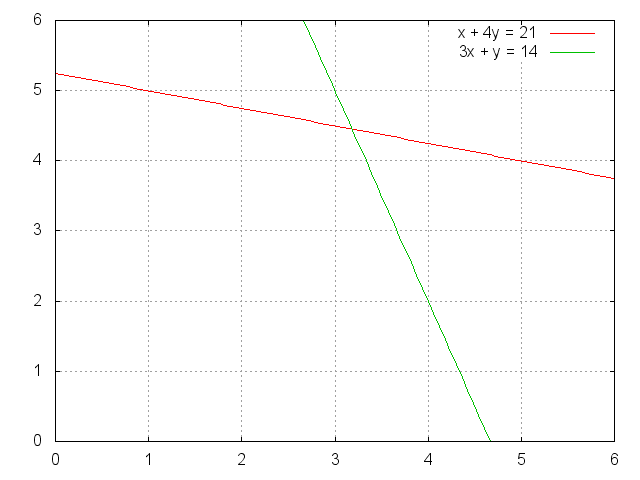
\includegraphics[scale=0.35]{ilpsample0.png}
\end{figure}

\end{frame} 

\begin{frame} 
\frametitle{Programaci�n lineal entera}

La b�squeda del �ptimo ya no debe hacerse sobre los v�rtices del poliedro, sino sobre los puntos enteros contenidos en �l.

\begin{figure}[h]
	\centering
	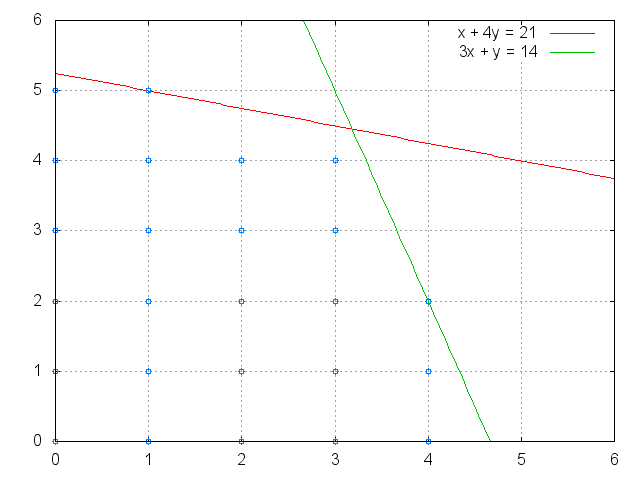
\includegraphics[scale=0.35]{ilpsample1.png}
\end{figure}

\end{frame} 

\begin{frame} 
\frametitle{Programaci�n lineal entera}

La b�squeda del �ptimo ya no debe hacerse sobre los v�rtices del poliedro, sino sobre los puntos enteros contenidos en �l.

\begin{figure}[h]
	\centering
	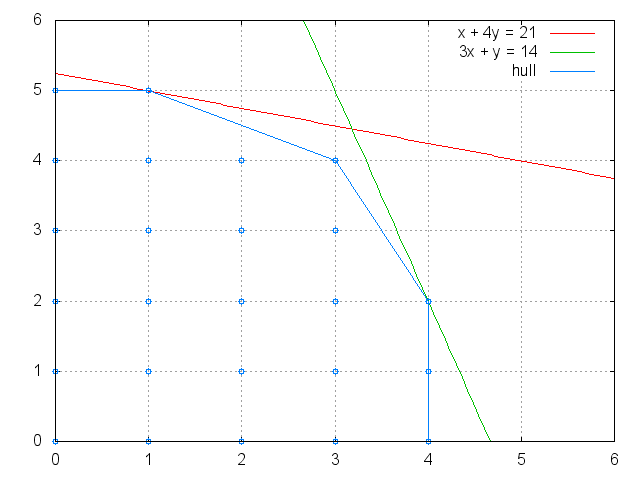
\includegraphics[scale=0.35]{ilpsample2.png}
\end{figure}

\end{frame} 

\begin{frame} 
\frametitle{Programaci�n lineal entera}

La b�squeda del �ptimo ya no debe hacerse sobre los v�rtices del poliedro, sino sobre los puntos enteros contenidos en �l.

\begin{figure}[h]
	\centering
	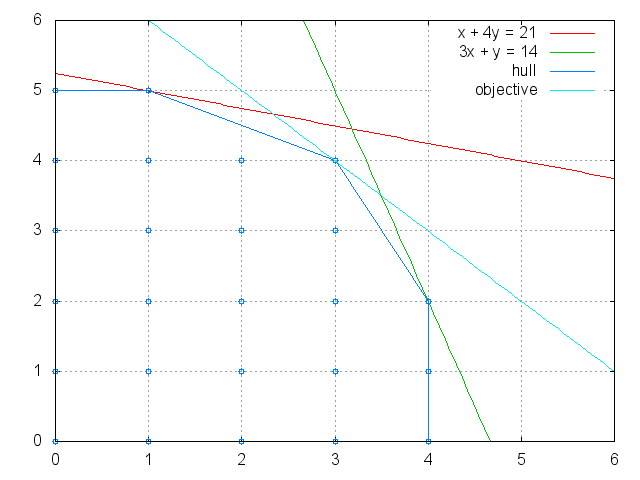
\includegraphics[scale=0.35]{ilpsample3.png}
\end{figure}

\end{frame} 

\begin{frame}
\frametitle{Programaci�n lineal entera}

A diferencia de programaci�n lineal con variables continuas, no se conoce algoritmo \textit{polinomial} para lineal entera.

Entre las t�cnicas para resolver este tipo de problemas se encuentran los algoritmos de \textit{branch and cut}, como el que aplicamos en este trabajo.

\end{frame}
